\chapter{Evaluation and Result Analysis}\label{ch:eval}

This chapter reports the completed Vermont benchmark comparison for the selected
controllers. The tables and figures in this chapter are drawn from the exported
\texttt{results}, \texttt{wandb}, and \texttt{target\_folder} outputs, together
with the consolidated summary generated by
\texttt{summarize\_selected\_experiment\_metrics}. Compared with the earlier
debugging-stage runs, the current result set is mature enough for a structured
comparison of tracking, comfort, peak demand, ramping, fairness, and
communication design.

\section{Evaluation Scope}

The experiments use the Annex 96 Common Exercise 1 CityLearn portfolios. Each
portfolio contains 25 single-family homes with photovoltaic generation and
battery storage. In the current report, the fully summarized comparison is the
Vermont setting, where January is used for training and February is used for
testing. Texas remains future work for the RL comparison, so the conclusions in
this chapter should be read as Vermont benchmark conclusions rather than
cross-climate conclusions.

\begin{table}[h]
\begin{center}
\begin{tabular}{|l|l|l|l|}
\hline
Climate & Training month & Testing month & Current status \\
\hline
Vermont & January & February & selected benchmark runs completed \\
Texas & August & September & RL comparison remains future work \\
\hline
\end{tabular}
\end{center}
\caption{Annex 96 train/test split and current evaluation scope.}
\label{tab:split}
\end{table}

The summarized Vermont comparison includes the main learned controllers used in
the project: standard MAPPO, grouped MAPPO, several grouped communication
variants, RLlib independent PPO, RLlib SAC rerun, and the RBC baseline. Most
MAPPO-based final runs use 500 training episodes in the selected set. The
comparison therefore no longer depends on the old pilot outputs.

\section{Main Vermont Results}

The primary objective is portfolio-level reference tracking. Let $y_t$ be the
actual aggregate portfolio load and $r_t$ be the reference load. The two main
tracking metrics are NMBE and CV-RMSE:

\begin{equation}
\mathrm{NMBE} =
\frac{\frac{1}{T}\sum_{t=1}^{T}(y_t-r_t)}
{\frac{1}{T}\sum_{t=1}^{T}r_t} \times 100\%,
\end{equation}

\begin{equation}
\mathrm{CV\mbox{-}RMSE} =
\frac{\sqrt{\frac{1}{T}\sum_{t=1}^{T}(y_t-r_t)^2}}
{\frac{1}{T}\sum_{t=1}^{T}r_t} \times 100\%.
\end{equation}

Lower absolute NMBE and lower CV-RMSE mean better tracking. Comfort exceedance
hours are also reported because a controller that tracks well but creates many
comfort violations is not practically useful.

Table~\ref{tab:vt-main-results} summarizes the main Vermont comparison. The
overall rank is taken from the consolidated summary table and combines the main
tracking metrics with selected secondary objectives.

\begin{table}[h]
\scriptsize
\begin{center}
\begin{tabular}{|l|r|r|r|r|r|}
\hline
Controller & Overall rank & CV-RMSE (\%) & $|$NMBE$|$ (\%) & Comfort hours & Reward sum \\
\hline
RBC baseline & 15 & 138.27 & 109.37 & 11465 & -- \\
RLlib Independent PPO & 4 & 51.78 & 21.84 & 10627 & -79395.8 \\
Standard MAPPO & 6 & 52.47 & 19.94 & 8809 & -13104.4 \\
Grouped MAPPO & 14 & 56.48 & 20.21 & 8100 & -27192.3 \\
Grouped Comm v2 & 1 & 49.94 & 17.74 & 7981 & -22907.9 \\
TarMAC & 5 & 50.92 & 18.56 & 8213 & -24165.3 \\
Weighted ($\alpha=0.90,\beta=0.10$) & 2 & 52.25 & 18.93 & 8451 & -26034.5 \\
GAT & 9 & 56.10 & 16.62 & 7882 & -21774.5 \\
PowerNet & 7 & 55.41 & 19.16 & 8100 & -27805.0 \\
DIAL & 13 & 65.51 & 29.10 & 11239 & -114468.5 \\
\hline
\end{tabular}
\end{center}
\caption{Completed Vermont benchmark comparison for representative controllers.}
\label{tab:vt-main-results}
\end{table}

\begin{figure}[h]
\begin{center}

\includegraphics[width=0.92\textwidth]{figures/selected_experiment_primary_metrics.png}
\end{center}
\caption{Primary metric summary generated from the selected Vermont experiment set.}
\label{fig:primary-summary}
\end{figure}

The mature Vermont comparison now shows a clearer pattern than the earlier
debugging-stage runs. First, grouped MAPPO with \texttt{comm\_v2} is the strongest overall
controller in the selected benchmark set: it is ranked first overall and first
on the primary ranking table, with the best CV-RMSE (49.94\%) and strong
comfort performance. Second, TarMAC is the strongest learned-attention variant
and is the closest competitor to \texttt{comm\_v2} on the primary metrics.
Third, the weighted communication variant with \mbox{$\alpha=0.90,\beta=0.10$}
is competitive and ranks second overall, showing that a stronger same-group
message can be helpful.

At the same time, the comparison also shows why one metric alone is not enough.
Standard MAPPO has the best reward sum among the learned controllers in
Table~\ref{tab:vt-main-results}, but it is not the best tracking controller.
RLlib independent PPO gives good CV-RMSE and strong peak reduction, but its
comfort hours are much worse than the main MAPPO variants. GAT has the lowest
absolute NMBE and the fewest comfort exceedance hours among the learned methods,
but its CV-RMSE and overall rank are weaker than the top communication methods.

\begin{figure}[h]
\begin{center}
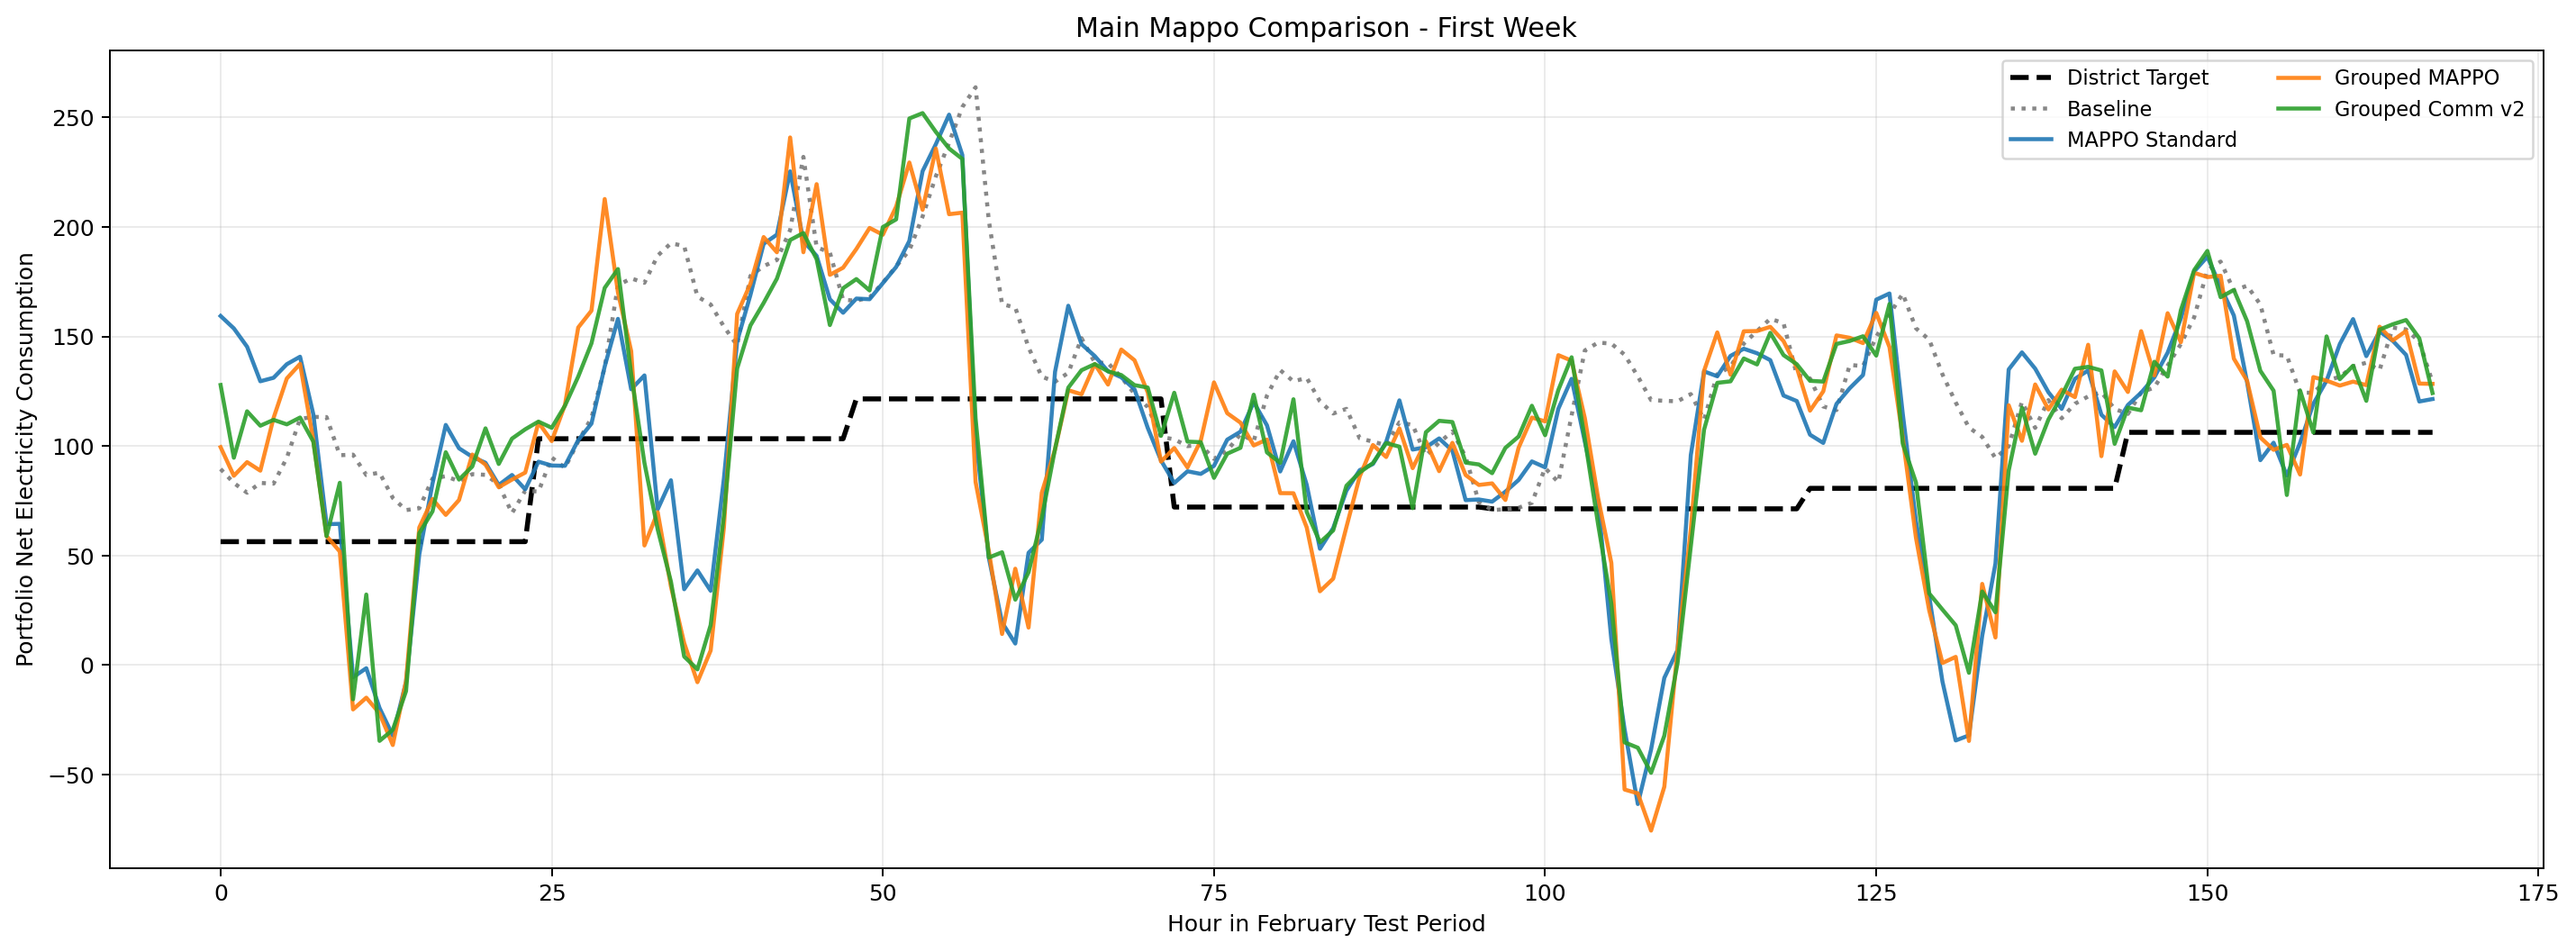
\includegraphics[width=0.92\textwidth]{figures/main_mappo_comparison_week1.png}
\end{center}
\caption{Week-1 aggregate load tracking for standard MAPPO, grouped MAPPO, and grouped Comm v2.}
\label{fig:main-mappo-week1}
\end{figure}

Figure~\ref{fig:main-mappo-week1} helps explain the main MAPPO comparison. The
grouped controller with \texttt{comm\_v2} follows the target more closely during
the visible high-load periods than standard MAPPO and grouped MAPPO without the
enhanced communication design. This visual pattern is consistent with its better
CV-RMSE in Table~\ref{tab:vt-main-results}.

\section{Communication Variant Comparison}

Table~\ref{tab:vt-comm-results} focuses on the communication variants. In
addition to the main tracking metrics, it includes peak-demand change and
fairness Gini so that the ranking can be interpreted as a trade-off rather than
as a single-number contest.

\begin{table}[h]
\scriptsize
\begin{center}
\begin{tabular}{|l|r|r|r|r|r|r|}
\hline
Method & Overall rank & Primary rank & CV-RMSE (\%) & Comfort hours & Peak change (\%) & Gini \\
\hline
Comm v2 & 1 & 1 & 49.94 & 7981 & -2.10 & 0.1796 \\
TarMAC & 5 & 2 & 50.92 & 8213 & -4.47 & 0.1564 \\
Weighted ($0.90,0.10$) & 2 & 5 & 52.25 & 8451 & -5.14 & 0.1784 \\
Weighted default & 11 & 4 & 55.05 & 8147 & -7.74 & 0.1906 \\
PowerNet & 7 & 6 & 55.41 & 8100 & -8.90 & 0.1784 \\
GAT & 9 & 3 & 56.10 & 7882 & -2.72 & 0.1276 \\
DIAL & 13 & 13 & 65.51 & 11239 & -10.88 & 0.1450 \\
\hline
\end{tabular}
\end{center}
\caption{Completed Vermont comparison for communication variants.}
\label{tab:vt-comm-results}
\end{table}

\begin{figure}[h]
\begin{center}

\includegraphics[width=0.92\textwidth]{figures/communication_method_comparison_week1.png}
\end{center}
\caption{Week-1 load tracking comparison for the main communication variants.}
\label{fig:comm-week1}
\end{figure}

Three communication conclusions are now supported by the completed Vermont
results. First, \texttt{comm\_v2} is the strongest all-round communication
variant in the current benchmark set. Second, TarMAC is the strongest
attention-based method and remains competitive on both tracking and comfort.
Third, communication quality depends strongly on design: DIAL performs poorly in
this task, while GAT gives very good comfort and fairness but weaker global
tracking.

The communication results also show that better peak reduction does not always
mean better overall control. PowerNet and DIAL reduce peak demand more strongly
than \texttt{comm\_v2}, but their CV-RMSE or comfort performance is worse. This
is why the combined ranking prefers \texttt{comm\_v2}, TarMAC, and the stronger
same-group weighted setting over those variants.

\section{Weighted Communication Ablation}

The weighted communication family is useful because it isolates one design
choice: how strongly the controller should favor same-group messages over
messages from the rest of the portfolio. Table~\ref{tab:weighted-ablation}
compares the three exported weighted settings.

\begin{table}[h]
\scriptsize
\begin{center}
\begin{tabular}{|l|r|r|r|r|}
\hline
Weighted setting & CV-RMSE (\%) & Comfort hours & Peak change (\%) & System ramping (kW) \\
\hline
Default ($0.75,0.25$) & 55.05 & 8147 & -7.74 & 460.7 \\
$\alpha=0.90,\beta=0.10$ & 52.25 & 8451 & -5.14 & 430.1 \\
$\alpha=0.55,\beta=0.45$ & 52.58 & 8561 & -9.79 & 439.4 \\
\hline
\end{tabular}
\end{center}
\caption{Weighted communication ablation in the completed Vermont comparison.}
\label{tab:weighted-ablation}
\end{table}

\begin{figure}[h]
\begin{center}
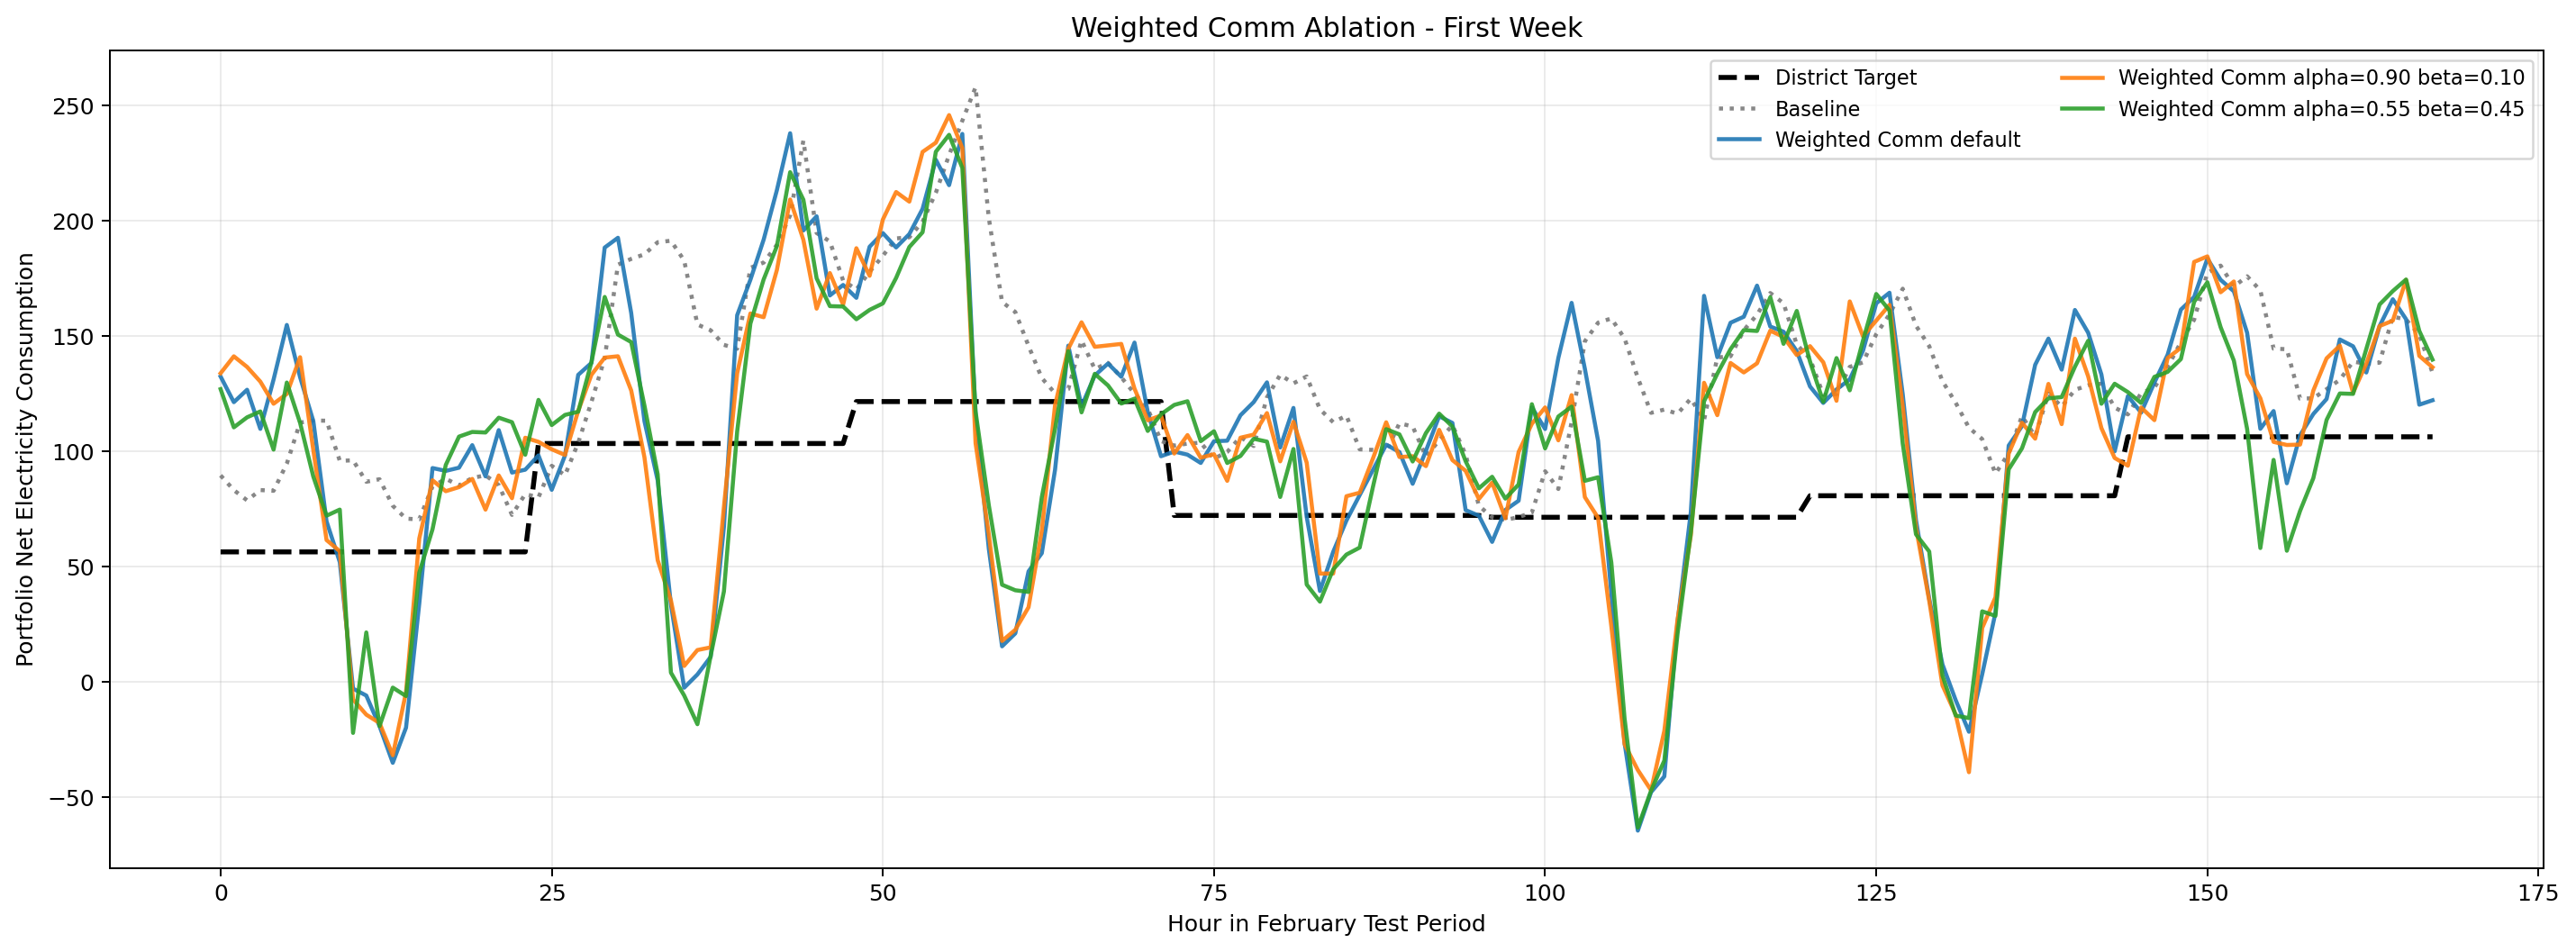
\includegraphics[width=0.92\textwidth]{figures/weighted_comm_ablation_week1.png}
\end{center}
\caption{Week-1 load tracking comparison for the weighted communication ablation.}
\label{fig:weighted-ablation-week1}
\end{figure}

The weighted ablation suggests that stronger same-group emphasis is a reasonable
direction. The \mbox{$\alpha=0.90,\beta=0.10$} setting has the best tracking of
the three weighted variants and also the lowest system ramping. The more
balanced \mbox{$\alpha=0.55,\beta=0.45$} setting gives the strongest peak
reduction, but its tracking and comfort are slightly worse. The default setting
is no longer the best weighted choice in the completed result set.

\section{Rule-Based Baseline}

Table~\ref{tab:rbc-baseline-results} reports the available RBC notebook
comparison for Texas and Vermont. The RBC baseline is still useful as a
non-learning reference, but it is clearly weaker than the learned Vermont
controllers on the CE1 load-tracking task.

\begin{table}[h]
\small
\begin{center}
\begin{tabular}{|l|r|r|r|r|}
\hline
Climate & NMBE RBC (\%) & NMBE baseline (\%) & CV-RMSE RBC (\%) & CV-RMSE baseline (\%) \\
\hline
TX & 89.57 & 79.12 & 207.63 & 163.74 \\
VT & 103.93 & 101.11 & 129.09 & 144.56 \\
\hline
\end{tabular}
\end{center}
\caption{RBC notebook baseline comparison against the CE1 target profile.}
\label{tab:rbc-baseline-results}
\end{table}

The RBC results show that fixed hour-based charging and discharging rules are
not enough for the CE1 objective. In Vermont, RBC improves CV-RMSE relative to
the no-control baseline, but its bias remains extremely large. In Texas, RBC is
worse than the no-control baseline on both NMBE and CV-RMSE. This supports the
use of learned controllers that respond to the target profile and to
portfolio-level conditions rather than following a fixed schedule.

\section{Secondary Metrics and Interpretation}

The secondary metrics add important context to the main ranking. For example,
RLlib independent PPO achieves a strong peak-demand reduction of 11.49\%, but
its comfort hours are far worse than the best MAPPO variants. GAT gives the
best fairness Gini in the selected set and also the lowest learned-controller
comfort hours, but its CV-RMSE is not competitive with the top two methods.
PowerNet and weighted communication reduce peak demand more strongly than
\texttt{comm\_v2}, but they do not match its combined tracking and comfort
balance.

Cost and carbon metrics are still not interpretable in the current exports
because the CE1 schemas used here do not provide pricing or carbon-intensity
files. CityLearn fills the missing signals with zero series, so the resulting
cost and carbon values are zero or null rather than meaningful control
outcomes.

\section{Current Interpretation and Remaining Limits}

The completed Vermont benchmark results support four conclusions. First, MARL is
useful for this task: the strongest MAPPO variants clearly outperform the RBC
baseline and avoid the very poor comfort trade-off seen in the independent PPO
baseline. Second, communication does matter, but it is not automatically
beneficial. Different communication designs create different trade-offs, and the
best result comes from a communication structure that is neither the simplest
nor the most complicated. Third, the best current Vermont controller is grouped
MAPPO with \texttt{comm\_v2}. Fourth, the weighted and attention-based variants
show that communication structure is a real optimization direction rather than a
minor implementation detail.

The remaining limits are now different from the earlier midterm stage. The
selected Vermont runs are complete, but the comparison still uses one seed and
one climate. Texas RL experiments, multi-seed validation, and cross-algorithm
comparison with methods such as MASAC or value-based approaches are still needed
before making broader claims about the full research question.
